\newpage
\subsection{Diagramma UML delle classi}
In questa sezione sono stati riportati tre diagrammi delle classi: il primo, in Figura \ref{fig:Initial Class diagram}, rappresenta il diagramma delle classi realizzato come prototipo per la progettazione dell'applicazione, il secondo, in Figura \ref{fig:Class diagram}, rappresenta il diagramma delle classi effettivamente ottenuto a seguito della stesura del codice dell'applicazione, mentre il terzo, in Figura \ref{fig:Simplified Class Diagram} rappresenta una versione semplificata del diagramma delle classi. In quest'ultima versione, in particolare, sono state rimosse alcune dipendenze in modo tale da rendere la comprensione di alcune relazioni tra classi visivamente più agevole.

Si tenga inoltre conto del fatto che le classi:
\begin{itemize}
    \item CampoNativo
    \item Categoria
    \item Configuratore
    \item Gerarchia
    \item User
    \item UserDataStore
\end{itemize}
implementano l'interfaccia \texttt{Serializable}, nonostante tale relazione non sia esplicitamente riportata nei diagrammi delle classi al fine di semplificare il layout dei diagrammi stessi.

\begin{figure}[hb]
    \centering
    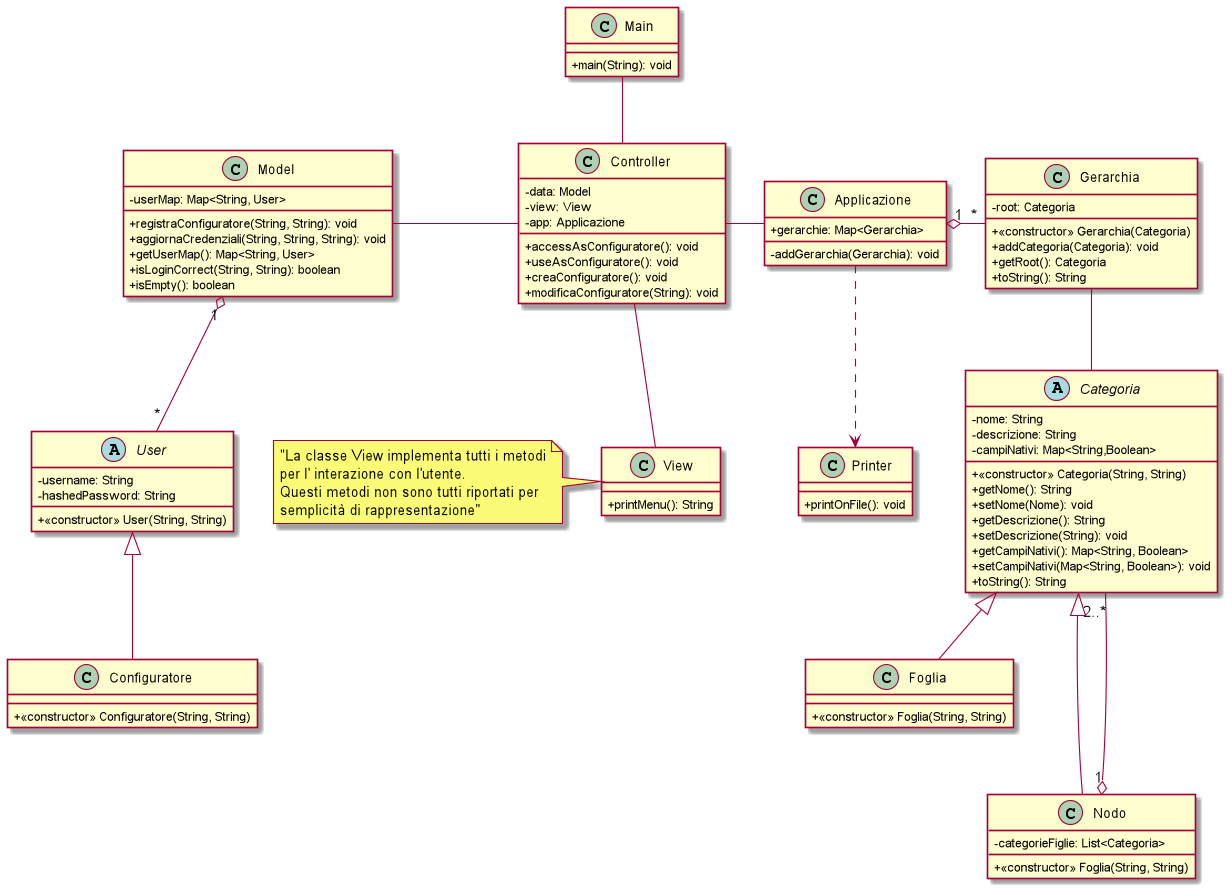
\includegraphics[width=\textwidth]{imagesV1/Initial class diagram - Version 1.0.png}
    \caption{\label{fig:Initial Class diagram}Prototipo di diagramma UML delle classi - Versione 1}
\end{figure}

\begin{figure}[h!]
    \centering
    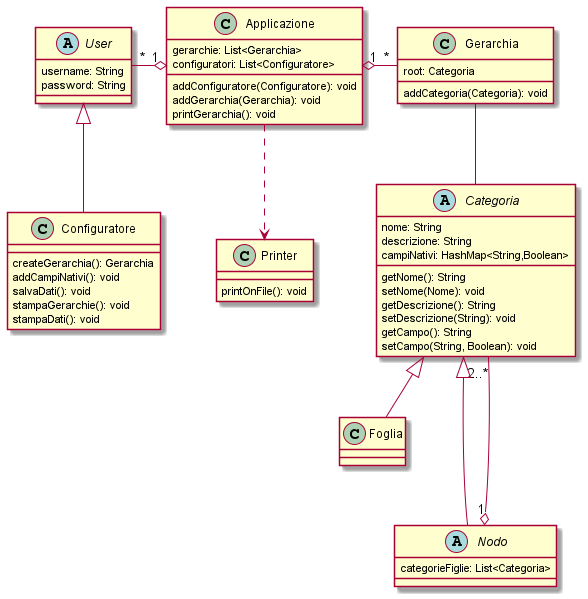
\includegraphics[width=\textwidth]{imagesV1/Class diagram-Version1.0.png}
    \caption{\label{fig:Class diagram}Diagramma UML delle classi - Versione 1}
\end{figure}    

La classe \texttt{View} contiene tutti i metodi (non indicati per esteso nel diagramma delle classi realizzato prima dell'effettiva stesura del codice) necessari per interagire e comunicare con l'utente, ricevendo i dati da lui inseriti oppure comunicando messaggi da parte del sistema.

La classe \texttt{Model}, presente con questo nome nell'UML iniziale ma rinominata \texttt{UserDataStore} nel codice finale, contiene i metodi necessari per la gestione dei dati relativi agli utenti che dovranno poi essere salvati in modo persistente. La classe ha il compito di gestire la registrazione di un nuovo utente Configuratore, l'aggiornamento delle credenziali e la verifica della correttezza delle informazioni introdotte in fase di login, oltre al salvataggio e al caricamento dei dati. 

La classe \texttt{User} è una classe astratta estesa dalla classe \texttt{Configuratore}: ogni Configuratore sarà dotato di username e password. La password, in particolare, viene salvata direttamente dopo aver effettuato l'hashing, in modo da garantire un livello di sicurezza basilare relativamente alle informazioni private degli utenti. La classe \texttt{User} è dotata di metodi per l'autenticazione dell'utente e per la modifica delle credenziali.

La classe \texttt{Applicazione} permette di tenere traccia delle gerarchie contenute nell'applicazione. 
Essa contiene infatti un metodo che verifica se il nome di una categoria radice di una gerarchia è già utilizzato dalla categoria radice di un'altra gerarchia, uno che permette di aggiungere una nuova gerarchia, metodi che permettono di ottenere le gerarchie presenti nell'applicazione o di assegnare loro i valori desiderati, metodi che permettono di salvare i dati contenuti nelle gerarchie e di caricare i dati salvati durante gli utilizzi precedenti dell'applicazione.

La classe \texttt{Gerarchia} permette di tenere traccia del contenuto di ogni gerarchia: ogni gerarchia è caratterizzata da una categoria radice che, a seconda che sia istanza della classe \texttt{Foglia} o \texttt{Nodo}, può avere o meno delle sottocategorie (a loro volta istanze della classe \texttt{Foglia} o \texttt{Nodo}). 

La classe \texttt{Categoria} è una classe astratta che è estesa dalla classe \texttt{Foglia} e dalla classe \texttt{Nodo}. Ogni categoria è dotata di nome obbligatorio, descrizione facoltativa e un insieme di campi nativi (due dei quali presenti di default per la categoria radice di una gerarchia) ereditati poi da ogni categoria figlia di un nodo.
La classe \texttt{Nodo}, in particolare, è dotata di una lista di categorie figlie che possono a loro volta essere foglie o nodi. Per questo motivo la classe \texttt{Nodo} è dotata di metodi che permettono di aggiungere o rimuovere una categoria figlia e di un metodo che permette di ottenere tutte le categorie figlie.

La classe \texttt{CampoNativo} tiene traccia dell'obbligatorietà della compilazione di un campo nativo o ereditato relativo a una categoria e del tipo del campo (di default si tratta di stringhe). 

La classe \texttt{CategoriaEntry} tiene traccia dell'associazione tra una categoria e la sua categoria padre; essa contiene pertanto i metodi necessari a recuperare le informazioni relative a tale relazione (percorso dalla categoria radice alla categoria corrente, categoria padre e categoria corrente) e dei metodi per trasformare una categoria da Foglia a Nodo e associarla alla propria categoria padre.

La classe \texttt{Controller} contiene metodi per consentire l'accesso a un profilo Configuratore, differenziando tra il caso di registrazione e quello di accesso standard. Ognuno di questi metodi richiama poi uno o più ulteriori metodi che permettono l'utilizzo delle funzionalità a cui l'utente è autorizzato ad accedere.

La classe \texttt{Main} contiene il solo metodo main che permette di interagire con l'applicazione selezionando l'azione da compiere tra accesso, registrazione o uscita dall'applicazione.

\begin{figure}[!]
    \centering
    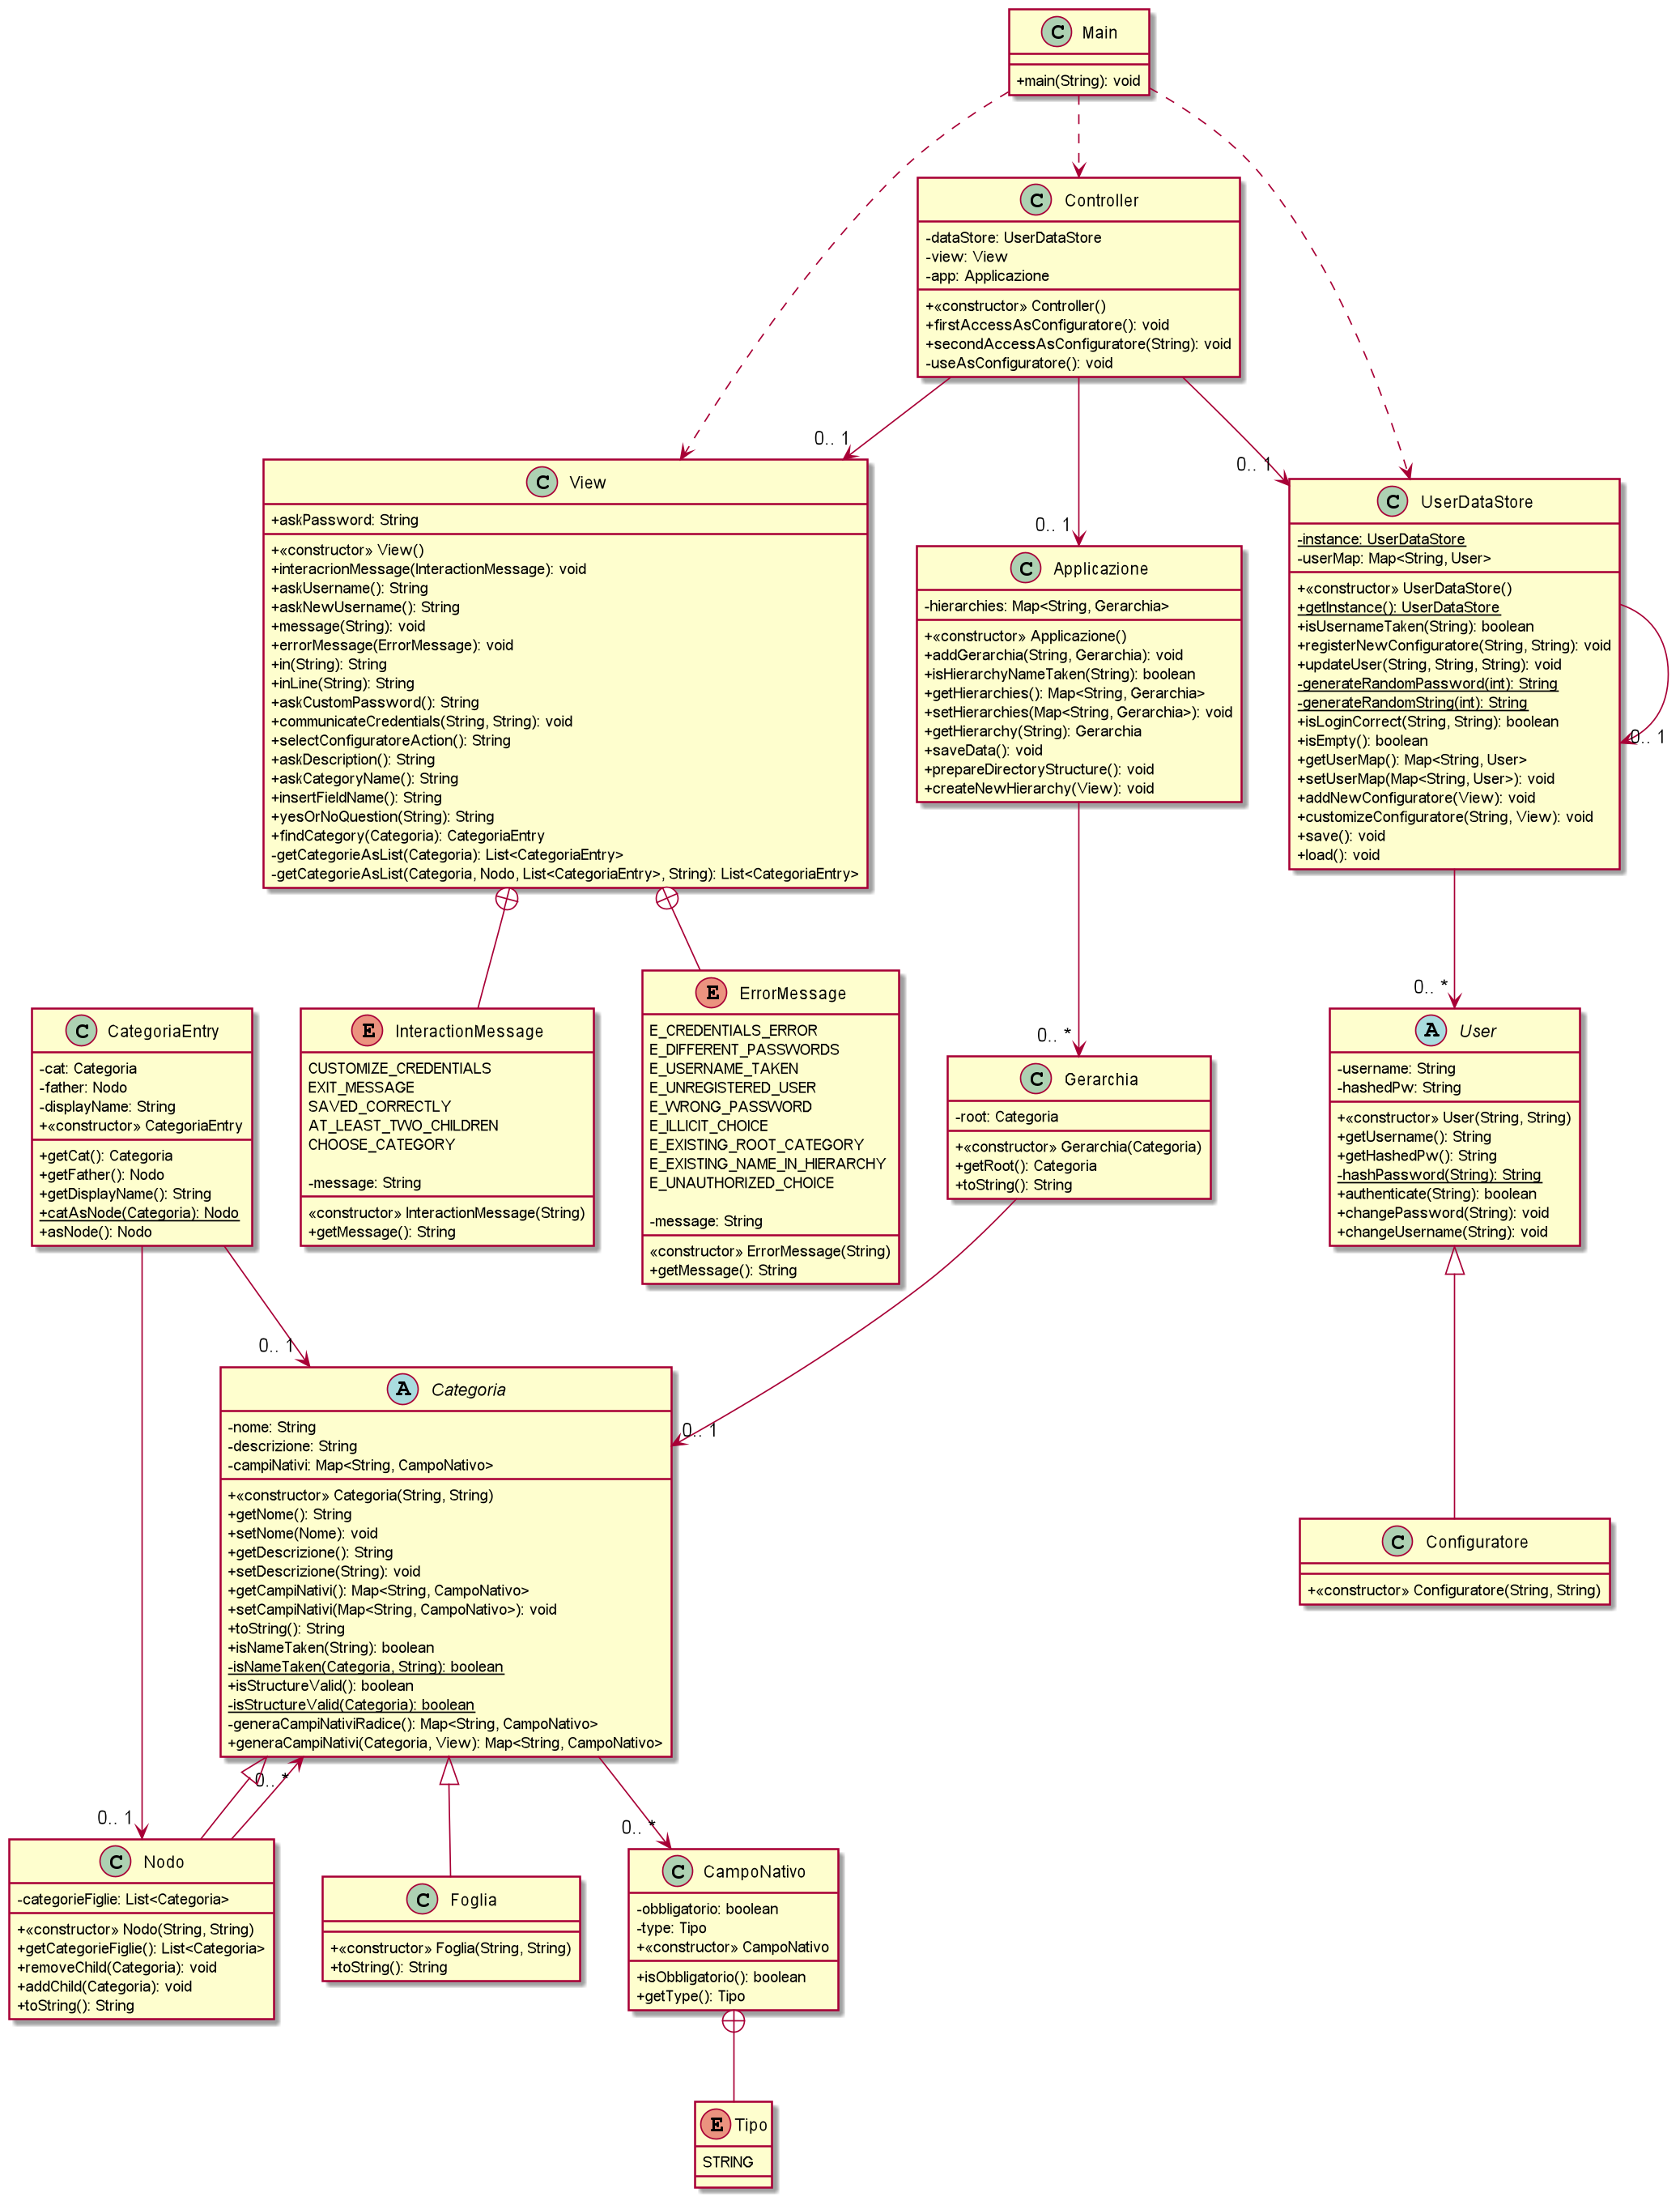
\includegraphics[width=\textwidth]{imagesV1/Class diagram simplified-Version1.0.png}
    \caption{\label{fig:Simplified Class Diagram}Diagramma UML delle classi semplificato - Versione 1}
\end{figure}